%%%%%%%%%%%%%%%%%%%%%%%%%%%%%%%%%%%%%%%%%%%%%%%%%%%%%%%%%%%%%%%%%%%%%%%%%%%%%%%%
%%%%%%%%%%%%%%%%%%%%%%%%% TOGGLES, CONSTANTS, SETTINGS %%%%%%%%%%%%%%%%%%%%%%%%%
%%%%%%%%%%%%%%%%%%%%%%%%%%%%%%%%%%%%%%%%%%%%%%%%%%%%%%%%%%%%%%%%%%%%%%%%%%%%%%%%

\newcount\Chatty  % whether to show our notes-to-selves in the pdf
\newcount\Drafty  % whether to show a timestamp in the pdf
\Chatty  = 1 % 0 for final copy; 1 for draft
\Drafty  = 1 % 0 for final copy; 1 for draft

%%%%%%%%%%%%%%%%%%%%%%%%%%%%%%%%%%%%%%%%%%%%%%%%%%%%%%%%%%%%%%%%%%%%%%%%%%%%%%%%
%%%%%%%%%%%%%%%%%%%%%%%%% DOCUMENT CLASS AND PACKAGES %%%%%%%%%%%%%%%%%%%%%%%%%%
%%%%%%%%%%%%%%%%%%%%%%%%%%%%%%%%%%%%%%%%%%%%%%%%%%%%%%%%%%%%%%%%%%%%%%%%%%%%%%%%

\documentclass[article,twocolumn]{memoir}
%\usepackage[utf8]{inputenc} % apparently not needed
\usepackage{amsmath}
\usepackage{amssymb}
\usepackage{amsthm}
\usepackage[calc, useregional, showseconds=false, showzone=false]{datetime2}
% also needs a line like the following in the file latexmkrc:
% $ENV{'TZ'}='America/New_York';
% ugh, except GitHub Actions won't respect that so instead we're setting the
% timezone to UTC and then doing black magic here in the latex source to compute
% the timezone.
\usepackage[table]{xcolor} % used in chatty macros
\usepackage{tikz}
\usepackage{graphicx}
\usepackage{hyperref}
\hypersetup{colorlinks=true,urlcolor=blue}
\usepackage{emoji}
%\usepackage{decorule} % makes a cool squiggly divider
%\usepackage{fourier-orns} % for fancy decorations
%\usepackage{pgfornament} % thing I tried for fancy decorations
\usepackage{float}
\usepackage[english]{babel}      % Apparently these 3 lines are the trick for
\usepackage[autostyle]{csquotes} %   letting you type quotes "like this" instead
\MakeOuterQuote{"}               %   of the LaTeX style ``like this''.
%\usepackage[normalem]{ulem}     % Underlining? Did Wamba need this?
\usepackage{flushend}            % Balance the columns on the last page

%%%%%%%%%%%%%%%%%%%%%%%%%%%%%%%%%%%%%%%%%%%%%%%%%%%%%%%%%%%%%%%%%%%%%%%%%%%%%%%%
%%%%%%%%%%%%%%%%%%%%%%%%%%%%% COMMANDS AND MACROS %%%%%%%%%%%%%%%%%%%%%%%%%%%%%%
%%%%%%%%%%%%%%%%%%%%%%%%%%%%%%%%%%%%%%%%%%%%%%%%%%%%%%%%%%%%%%%%%%%%%%%%%%%%%%%%

\newcommand{\dreev} [1]{\ifnum\Chatty=1 \textcolor{red} {dreev:  [#1]} \fi}
\newcommand{\wamba} [1]{\ifnum\Chatty=1 \textcolor{blue}{wamba:  [#1]} \fi}
% Available colors: red, blue, purple, orange, teal, etc

% Utter black magic for doing timezone conversion for the draft timestamp...
% Via https://tex.stackexchange.com/questions/634804/how-to-change-the-timezone
\newcommand{\datetimemagic}[2]{\DTMsavenow{now}\DTMtozulu{now}{cz}
  \DTMsaveaszulutime{cx}{\DTMfetchyear{cz}}{\DTMfetchmonth{cz}}
  {\DTMfetchday{cz}}{\DTMfetchhour{cz}}{\DTMfetchminute{cz}}
  {\DTMfetchsecond{cz}}{#2}{00}\DTMdisplay{\DTMfetchyear{cx}}
  {\DTMfetchmonth{cx}}{\DTMfetchday{cx}}{}{\DTMfetchhour{cx}}
  {\DTMfetchminute{cx}}{\DTMfetchsecond{cx}}{#1}{00}}
% And here's even more unDRY ugliness because I don't know what I'm doing...
\newcommand{\datemagic}[2]{\DTMsavenow{now}\DTMtozulu{now}{cz}
  \DTMsaveaszulutime{cx}{\DTMfetchyear{cz}}{\DTMfetchmonth{cz}}
  {\DTMfetchday{cz}}{\DTMfetchhour{cz}}{\DTMfetchminute{cz}}
  {\DTMfetchsecond{cz}}{#2}{00}\DTMdisplaydate{\DTMfetchyear{cx}}
  {\DTMfetchmonth{cx}}{\DTMfetchday{cx}}{}}

% Set this to, eg, -08/+08 for Pacific Time in winter, -07/+07 in summer. Woof.
\newcommand{\tstamp}{\ifnum\Drafty=1 
  \textcolor{red}{DRAFT~\datetimemagic{-07}{+07}} \else 
  \datetimemagic{-07}{+07}
\fi}

\newcommand{\snakedivider}{
\vspace{.2em}
\begin{center}
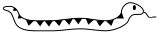
\includegraphics[width=.25\linewidth]{snake}
\end{center}
\vspace{.1em}
}
% Other divider lines I've tried out:
%\begin{center}\pgfornament[scale=.18]{85}\end{center}\vspace{.5em}
%\begin{center}\decorule\end{center}
%\vspace{1em}
%\fancybreak{\decofourleft \quad \decofourright}
%\vspace{1em}
%\begin{center}\emoji{thought-balloon}\end{center}
%\vspace{1em}
%\vspace{1em}
% SCHDEL:
%\usetikzlibrary{decorations.pathmorphing}
%\newcommand{\squigglyline}{
%\begin{center}
%\begin{tikzpicture}
%\pgfmathsetmacro\seglen{0.5*0.1}
%\draw [line width=0.4mm, decoration={snake, amplitude=1mm, segment length=\seglen\linewidth}, decorate] (0,0) -- (0.5\linewidth,0);
%\end{tikzpicture}
%\end{center}
%}


\hfuzz=2pt % Don't bother to report overfull hboxes if over-edge is < 2pt
\vfuzz=2pt % Same for overfull vboxes (maybe just works for hfuzz?)

%\newcommand{\BibTeX}{\rm B\kern-.05em{\sc i\kern-.025em b}\kern-.08em\TeX}

%%%%%%%%%%%%%%%%%%%%%%%%%%%%%%%%%%%%%%%%%%%%%%%%%%%%%%%%%%%%%%%%%%%%%%%%%%%%%%%%
%%%%%%%%%%%%%%%%%%%%%% TITLE, AUTHORS, ABSTRACT, KEYWORDS %%%%%%%%%%%%%%%%%%%%%%
%%%%%%%%%%%%%%%%%%%%%%%%%%%%%%%%%%%%%%%%%%%%%%%%%%%%%%%%%%%%%%%%%%%%%%%%%%%%%%%%

\newcommand{\longtitle}{The Snake Eyes Paradox}
\newcommand{\shorttitle}{A response to Lorxus' Questions for Team YES} % for page headers

\title{\HUGE\textbf{\longtitle}\\ \textbf{\shorttitle}}
\author{Daniel M. Reeves\\manifold.markets/dreev
\and
Wamba Ivanhoe\\manifold.markets/ShitakiIntaki
}
\date{\protect\tstamp} % need protection from black magic, apparently

%\begin{abstract}
%The answer is 1/36.
%\end{abstract}

%\keywords{Probability, Math puzzles}

%%%%%%%%%%%%%%%%%%%%%%%%%%%%%%%%%%%%%%%%%%%%%%%%%%%%%%%%%%%%%%%%%%%%%%%%%%%%%%%%
%%%%%%%%%%%%%%%%% START DOCUMENT, SET UP HEADERS, DO MAKETITLE %%%%%%%%%%%%%%%%%
%%%%%%%%%%%%%%%%%%%%%%%%%%%%%%%%%%%%%%%%%%%%%%%%%%%%%%%%%%%%%%%%%%%%%%%%%%%%%%%%

\begin{document}
\pagestyle{headings}
\maketitle

%%%%%%%%%%%%%%%%%%%%%%%%%%%%%%%%%%%%%%%%%%%%%%%%%%%%%%%%%%%%%%%%%%%%%%%%%%%%%%%%
%%%%%%%%%%%%%%%%%%%%%%%%%%%%%%%% MAIN DOCUMENT %%%%%%%%%%%%%%%%%%%%%%%%%%%%%%%%%
%%%%%%%%%%%%%%%%%%%%%%%%%%%%%%%%%%%%%%%%%%%%%%%%%%%%%%%%%%%%%%%%%%%%%%%%%%%%%%%%

\chapter*{Questions for Team YES}
\begin{itemize}
    \item Why should I believe that the “true” Snake Eyes setup, which is intrinsically infinitary, will behave nicely as a limit of its suitably defined (finite) initial segments? After all, there’s things that can happen in any finite case that never can - they’re literally impossible - or never will - they have probability 0 - in the infinitary case! The fact that your final expression for P r(death|chosen) has no N-dependence is a promising data point, but on its own it’s not enough.

    {\color{violet} 
        RESPONSE: 
        \wamba{Why doesn't Bartha Hitchcock paper look at the problem this way? This seems easier than constructing the non-standard analysis framework, so ostensibly there is a flaw in this approach as well, unless the non-standard analysis framework was only needed to reconcile the Shooting Room Paradox's $\frac{9}{10}$ and $\frac{1}{36}$ death rates since their preamble says that $\frac{1}{36}$ is correct in all cases}
        If we shift to looking at the probability of losing, if you are chosen in Round i, with out making any assumption about any finiteness of the game I believe we will have allowed for the intrinsically infinitary nature of the game.
        Let $\Pr(i,j)$ be the mutually exclusive absolute odds of an individual being selected in Round $i$ of a game that rolls snake eyes in Round $j$, let $\Pr(C_i)$ be the probability of being selected in Round $i$ and let $\Pr(E_j)$ be the probability of the game ending in snake-eyes rolled in Round $j$.

        Where
        $$\Pr(E_j) = p(1-p)^{j-1}$$
        This is precisely the odds of rolling $j-1$ not snake eyes results and then finally rolling snake eyes in the $j^\text{th}$ round and satisfies the countable additivity property of probability 
        $$\sum_{j=1}^\infty \Pr(E_j) =\sum_{j=1}^\infty p(1-p)^{j-1}= \frac{p}{1-(1-p)}=1$$
        
        Where
        $$\Pr(C_i) = \lim_{m\to\infty}\frac{2^{i-1}}{2^m-1}$$
        This represents the doubling population that plays in each successive round of the game, however the limit is an infinitesimal and in order to have a semblance of retaining the countable additivity property of probability we have to constrain the total population, which is ultimately infinite, to 1 less than a power of two, which we allow to grow with out bound in the limit to still have an infinite population. 
        $$\sum_{i=1}^\infty \Pr(C_i) = \lim_{m\to\infty}\sum_{i=1}^m\frac{2^{i-1}}{2^m-1}=\lim_{m\to\infty}\frac{2^m-1}{2^m-1}=1$$ 
        then
            \begin{align*}
              \Pr(i,j) & = \Pr(C_i)\Pr(E_j)\\
              \Pr(i,j) & = \Pr(C_i)p(1-p)^{j-1}
            \end{align*}
        We note that in the limit each $\Pr(C_i)$ is infinitesimal however the sum across all $C_i$ is still 1 in the limit.
        
        The sum of all possible $\Pr(i,j)$ is also 1 as a disjoint covering of the probability space.
        $$\sum_{i=1}^\infty\sum_{j=1}^\infty \Pr(i,j) =\sum_{i=1}^\infty \Pr(C_i)\sum_{j=1}^\infty\Pr(E_j) = 1 $$
        The sum of any subset of these disjoint $Pr(i,j)$ must therefore in all cases be within the range $[0,1]$, and actually we can refine this range to $(0,1]$ provided that we consider $i>j$ cases to be where you would have played in Round $i$ if the game had not ended in the earlier Round $j$.
        
        You only play in Round $i$ if $i\leq j$.  You die when $j=i$ otherwise you live for all $j>i$. 
            \begin{align*}
                 \Pr(E_i|C_i)&=\frac{\Pr(E_i\land C_i)}{\Pr(C_i)}\\ 
                 &=\frac{\Pr(i,i)}{\sum_{j=i}^\infty \Pr(i,j)}\\
                 &=\frac{\Pr(C_i)p(1-p)^{i-1}}{\sum_{n=i}^{\infty} \Pr(C_i)p(1-p)^{n-1}}\\
                 &=\frac{p(1-p)^{i-1}}{\sum_{n=i}^{\infty}p(1-p)^{n-1}}\\
                 &=\frac{p(1-p)^{i-1}}{p\frac{(1-p)^{i-1}}{1-(1-p)}}\\
                 &=\frac{p(1-p)^{i-1}}{(1-p)^{i-1}}\\
                 &=p
            \end{align*}
            Ergo the probability of dying in Round $i$, conditional on being chosen in Round $i$ is $p$.

        The absolute odds of dying is found by adding up all the possible games where we are selected in the final round:
        \begin{equation}
          \sum_{j=1}^{\infty} \Pr(j,j) \label{die}
        \end{equation} 
        The absolute odds of being chosen are the games where  $i\leq j \text{ }\forall \text{ } i\text{,}j \in \mathbf{N}$:
        \begin{equation}
          \sum_{j=1}^{\infty} \sum_{i=1}^{j} \Pr(i,j) = \sum_{i=1}^{\infty} \sum_{j=i}^{\infty} \Pr(i,j) \label{chosen} 
        \end{equation}
        
        The odds of dying, conditioned upon being selected is simply the ratio of eq. \ref{die} over eq. \ref{chosen}
        \begin{equation}
          \frac{\sum_{j=1}^{\infty} \Pr(j,j)}{\sum_{j=1}^{\infty} \sum_{i=1}^{j} \Pr(i,j)} = \frac{\sum_{i=1}^{\infty} \Pr(i,i)}{\sum_{i=1}^{\infty} \sum_{j=i}^{\infty} \Pr(i,j)}\label{theAnswer}
        \end{equation}

        Generally 
            $$\frac{\sum_{i=1}^{n} a_i}{\sum_{i=1}^{n} b_i}\nLeftrightarrow \sum_{i=1}^{n} \frac{a_i}{b_i}$$

        However we do know that if 
            $$\frac{a_i}{b_i}=\frac{a_j}{b_j} \text{   } \forall \text{ } i\text{,}j$$
        then
            $$\frac{\sum_{i=1}^{n} a_i}{\sum_{i=1}^{n} b_i} = \frac{a_j}{b_j}\text{   } \forall \text{ } i\text{,}j$$
        and we have just shown that 
            $$\frac{\Pr(i,i)}{\sum_{j=i}^\infty \Pr(i,j)} = p \text{   } \forall \text{ } i\text{,}j$$
        therefore 
            $$\frac{\sum_{i=1}^{\infty} \Pr(i,i)}{\sum_{i=1}^{\infty} \sum_{j=i}^{\infty} \Pr(i,j)}=p$$
    }


\item More broadly, there’s issues in how your write up handles expressions that roughly cash out as something like 0∗∞ - at the moment, it seems to tacitly assume that all such expressions should be evaluated as 0.
    
    {\color{violet}
        RESPONSE: 
        0*$\infty$ or 0/0 is undefined, not zero, in standard analysis setting which is why the YES write-up shifts to taking the limit of a finitary starting population.
    }
    \wamba{Need to re-read the YES write up to see what assumption evaluates expressions as 0.}
\item What conditions, if any, need to be placed on the finitary starting population size M in order to avoid problems when you pass to the infinitary case? Here I’m mostly worried about St. Petersburg’s Paradox-flavored problems.

   {\color{violet}
        RESPONSE:
        \begin{align*}
            \Pr(\text{chosen}) &= \sum_{i=1}^{N} \tfrac{1}{M} 2^{i-1}(1-p)^{i-1}\\
            &= \frac{1}{M} \sum_{i=1}^{N} \bigg(\frac{35}{18}\bigg)^{i-1}\\
            &= \frac{1}{M} \frac{1-\bigg(\frac{35}{18}\bigg)^{N}}{1-\frac{35}{18}}\\
            &= \frac{1}{M} \frac{18}{17}\bigg(\big(\frac{35}{18}\big)^N-1\bigg)
        \end{align*}
        can grow unbounded with $N$ if there are no conditions on the starting population size $M$.  The YES write up already conditions $M = 2^N-1$.  So by substitution of $M$
        $$\Pr(\text{chosen})= \frac{18}{17}\frac{\big(\frac{35}{18}\big)^N-1}{2^N-1} \text{  }\forall\text{  }N \in \mathbf{N}$$
        $\Pr(\text{chosen})$ clearly is not a quantity growing with out bound but rather is bound within the range 
        $$\frac{18}{17}\bigg(\frac{35}{36}\bigg)^N\geq \frac{18}{17}\frac{\big(\frac{35}{18}\big)^N-1}{2^N-1}  = \underset{\text{as }N\to\infty }{\text{infinitesimal}} \geq 0$$
        The constraint that $M = 2^N-1$ is sufficient, but not necessary. $M$ can be allowed to grow up to $2^{N+1}-2$, beyond this upper bound for $M$ we would have enough population to fill at least an $N+1$ cohort so if we are to say that $N$ is the upper bound of rounds we can play before we terminate then $M\geq 2^{N+1}-1$ would contradict this definition of $N$.

        Now we need to address the fact that when we divide by $\Pr(\text{chosen})$ in the context of the conditional probability it is equivalent to multiplying by $\infty$.

        \wamba{How do you get a St. Petersburg Paradox where you are looking exclusively at the odds, not at expected values?}
        \begin{align*}
            \Pr(\text{death})& = \sum_{i=1}^{N} \Pr(i,i)= \sum_{i=1}^{N} \tfrac{1}{M} 2^{i-1}p(1-p)^{i-1}\\
            & \text{by factoring out the constant factor p} \\
            & = p\Pr(\text{chosen})
        \end{align*}

        The numerator is approaching an infinitesimal quantity in at rate proportional to the the rate the denominator is approaching an infinitesimal quantity.  Their ratio is p.
    }
    
\item Suppose Team No’s objection to Clarification 3 - namely, that it’s incoherent due to under-specification - is spot-on, and you really do need to motivate bounded-escape over bounded death as the natural finitary analogue. How?

    {\color{violet}
        RESPONSE: 
        To motivate bounded-escape over bounded death as the natural finitary analogue, one looks only to the algorithm. The game described is non-adversarial, and the dice are independent, and the dice are rolled in every round.  Each round you take a disjoint cohort, roll the dice, if it is snake eyes you kill the cohort and stop recruiting any new cohorts because the game has ended, if it is not snake eyes the cohort lives(wins) and you proceed to recruit the next disjoint cohort.  To motivate the bounded-escape case you need only follow the algorithm until you cannot, Recruit a disjoint cohort, if you can, and roll the dice, repeat as necessary, any one who plays and lives, only lives because they observed non-snake eyes in their round. Whereas NO's bounded-death game introduces a new rule/mechanism which must necessarily ignore the roll of any dice for the final cohort, "If after recruiting a cohort it is apparent that there will be insufficient population left to recruit any further cohorts, then do not roll dice, just kill this cohort."  If you need a new rule which must supersede the previous "rule" that independent dice are rolled to determine the outcome of each round, then you have changed the game.
    }
\item What, precisely, should be meant by “chosen”? Chosen for round i? For at least one of the rounds? Something else?
    \wamba{I am not sure about the consequences of any of these,  with the reformulated by Chosen in Round $i$ if feel like we could shift to a Pr(chosen)=1 world such as, only minds which play exist.}
    {\color{violet}
        RESPONSE: 
        The game described is drawing from a population at random. The conditional question must then be over the total probability that you are drawn from the population at random. NO's position requires that the conditional event equal 1 in the absolute sense for it to work because they cannot address the lack of a uniform prior probability of being selected at random from a population with out non-standard analysis.  YES's position holds regardless if we are in a non-standard setting or a standard setting with a countably additive probability.
    }
    
        \wamba{[TOD?O: add countably additive probability in lieu of a non-standard uniform prior, steal from Bartha-Hitchcock]}
        
        \wamba{[Do we even need to choose from an infinite population?  What if we simply say. With probability 1, you play in Round $i$, then what are the odds that the game ends in Round $i$ vs the odds that the game ends in Round $j>i$, again we ignore all the $j<i$]}
\item How do you reconcile the fact that you get a value of $\frac{17}{18}$ for the probability of never rolling snake-eyes [conditioned upon being chosen] with the direct calculation of $\underset{n\to\infty}{\lim}1-\frac{35}{36}^n=1$

\wamba{per Lorxus: Yes, that is supposed to refer to the  probability of never rolling snake eyes conditioned upon being chosen. There's some algebra there but it's a little incomplete, and the narrative is lacking.}
    
    {\color{violet}
        RESPONSE: 
        \wamba{ This feels, increasingly, like blowing smoke. I am inclined to abandon everything at resort exclusively to the reformulated YES argument, constructed in the vein of NO's construction, in which case we might want to look at the NO questions and preemptively address such issues.}

        \wamba{ So with the clarification from Lorxus, I guess we just need to make the math easier to follow, and improve the narrative.}
        
        So the question is that if rolling snake eyes happens with probability of 1, how can the zero measure event of never rolling snake eyes be $\frac{17}{18}$.  The claim is not made in the naked context of absolute probability but rather conditioned upon the also zero measure event of having been chosen at random from the countably infinite population.

         $$\Pr(\text{chosen})= \lim_{n\to\infty}\frac{18}{17}\frac{\big(\frac{35}{18}\big)^n-1}{2^n-1}$$
         $$\Pr(\text{roll snake})=\underset{n\to\infty}{\lim}1-\bigg(\frac{35}{36}\bigg)^n=1$$
         $0<\bigg|\Pr(\text{rol snake)}-1\bigg|<\epsilon\text{,   }\forall\text{   } n>\frac{\ln{\epsilon}}{\ln{35}-\ln{36}}$
         $$\Pr(\text{never roll snake})=\lim_{n\to\infty}\bigg(\frac{35}{36}\bigg)^n$$
         \begin{align*}
             &\Pr(\text{never roll snake|chosen})\\
             &=\frac{\Pr(\text{never roll snake}\land\text{chosen})}{\Pr(\text{chosen})}\text{, or alternatively}\\
             &=\frac{\Pr(\text{chosen|never roll snake})\Pr(\text{never roll snake})}{\Pr(\text{chosen})}\\
             &=\frac{1 * \Pr(\text{never roll snake})}{\Pr(\text{chosen})}\\
             &=\frac{\lim_{n\to\infty}\bigg(\frac{35}{36}\bigg)^n}{\lim_{n\to\infty}\frac{18}{17}\frac{\big(\frac{35}{18}\big)^n-1}{2^n-1}} = \lim_{n\to\infty}\frac{17}{18}\frac{35^n(36^n-18^n)}{36^n(35^n-18^n)}\\
             %%&\text{for }\epsilon>0, \bigg|\Pr(\text{never roll snake|chosen})-\frac{17}{18}\bigg|<\epsilon\\
             %%&\forall \text{  }n>
             &=\frac{17}{18}
         \end{align*}
        
        Nearly every game ends in snake eyes before you are selected.  These games would fall outside of the probability space used to calculate the conditional probability of your death conditioned upon the unlikely even that you are chosen to play.   Of the games you are selected to play in, there are infinitely many games that end in snake eyes and therefor have a finite number of players, and there  games that, improbable as it may be, never rolls snake eyes.  If instead of thinking of it as 2d6 we think of it as a binary distribution with $p=\frac{1}{36}$ then we might say there is exactly one game that never ends
    }
\item You appear to start by postulating an already-existing countably infinite population to draw from, such that you can experience not having been chosen. Why is this relevant to a question for which having been chosen should be true by assumption? And if we do assume infinite starting population, why isn’t the answer immediately 0? I need to see some more discussion of how you handle infinities here.

    {\color{violet}
        RESPONSE: 
        
    }
\item Suppose we keep the Snake Eyes Game going forever, continuing to pull larger and larger (disjoint) cohorts from our countably infinite population and killing all and only the cohorts that roll snake-eyes. Is there anything different about the probabilities of this game’s expected outcomes for any given player? Why or why not?

    {\color{violet}
        RESPONSE: 
       
        We now in all cases have that the chance that you are chosen to play is 1, everyone plays.  On the one hand, for YES, we could look at the odds of rolling snake-eyes given that you are playing in Round $i$ and we would find that the player observes a single dice roll and therefore should have an expectation of $p$ for death.  The fact that everyone plays does not mess things up here for the YES rational.

        On the other hand, for NO, looking at the game from the perspective of the rounds which resulted in snake-eyes and therefore death, there are infinitely many snake eyes rounds in contrast to the original game's single game ending round, and there are infinitely many non-snake eyes rounds in contrast to the finitely(?) many non-snake rounds in the original game setting.  So we have $\frac{\infty}{\infty}$ which is undefined, but in this context we have no way of setting up any similitude of a limit in the standard analysis sense.

        Any given player plays with probability 1.  The game progressing to any particular round also has probability 1.  The "random" events are which round did you play in, and did that round roll snake eyes.  Did the round you play in result in snake eyes?  You can only play in one round since they are disjoint cohorts, so the possibility of death must be $p$.

        The NO argument might try to form a disjoint partition of the infinite population such that each partition contains exactly one round that resulted in snake eyes, and then argue that within each partition it is analogous to one of their summation terms, with the exception that the total number of players that played and died are scaled by some factor of $2^n$ such that the internal death rate within that partition that runs for n games since the prior snake eyes corresponds to the nth term of the summation, and similarly is weighted by the frequency of such runs of n length.
    }
\end{itemize}

\chapter*{Lorxus' Takaways}
As it stands, both of these writeups, while good, have some serious flaws and gaps in them. The ones I have noted here are only the first few that stood out to me on reading through. The major points of remaining confusion or disagreement that I see are two closely-related ones. 
\begin{itemize}
    \item The first is over the nature of the word “chosen” - if we construe it to mean something like “start with a countably infinite population and draw from it”, we get one answer, and if we construe it to mean “only minds that actually play some round of the Snake Eyes Game”, then we get another. 

        \wamba{So yeah I guess the NO formulation, assumes that "you" play in all games, so they take an average of all games. Any possible game has a finite end approaching 1/2.  But you have to play in some specific round so we can formulate YES around you play in Round i.}
    \item The second is over the nature of the starting population, and who among the set of all minds gets to count as having been chosen for the game - again, we could decide that this means that the entire infinite set of possible minds counts as having been chosen - they might enter the game, and in some universe any given mind does! - and we could also decide that this means that only some finite population that actually did pass through the game counts.
\end{itemize}
\end{document}